\documentclass[11pt]{article}
\usepackage[scaled=0.92]{helvet}
\usepackage{geometry}
\geometry{letterpaper,tmargin=1in,bmargin=1in,lmargin=1in,rmargin=1in}
\usepackage[parfill]{parskip} % Activate to begin paragraphs with an empty line rather than an indent %\usepackage{graphicx}
\usepackage{amsmath,amssymb, mathrsfs, dsfont}
\usepackage{mathtools}

\usepackage{tabularx}
\usepackage[font=footnotesize,labelfont=bf]{caption}
\usepackage{graphicx}
\usepackage{xcolor}
%\usepackage[linkbordercolor ={1 1 1} ]{hyperref}
%\usepackage[sf]{titlesec}
\usepackage{natbib}
\usepackage{../../Tianpei_Report}

%\usepackage{appendix}
%\usepackage{algorithm}
%\usepackage{algorithmic}

%\renewcommand{\algorithmicrequire}{\textbf{Input:}}
%\renewcommand{\algorithmicensure}{\textbf{Output:}}



\begin{document}
\title{Lecture 4: Dynamic Programming (DP)}
\author{Tianpei Xie}
\date{ Aug 2nd., 2022 }
\maketitle
\tableofcontents
\newpage
\section{Policy evaluation vs. Control}
In reinforcement learning, there are two major distinct tasks: \emph{policy evaluation} and \emph{control}:
\begin{itemize}
\item \textbf{Policy evaluation} or \textbf{\emph{Prediction}} is the task of determining the value function for a specific policy. Note that the value function is a prediction of future rewards, in terms of expected returns. Thus estimation of value function is a task of predicting future rewards. The prediction task is an \emph{unsupervised learning task}, since no human label is required and we just need to wait for the rewards. 

\item \textbf{Policy Improvement} or \textbf{\emph{Control}}  is the task of \textbf{finding a policy} to obtain as much reward as possible. In other words, finding a policy which \emph{maximizes} the value function.
\end{itemize}
\begin{figure}
\begin{minipage}[t]{1\linewidth}
  \centering
  \centerline{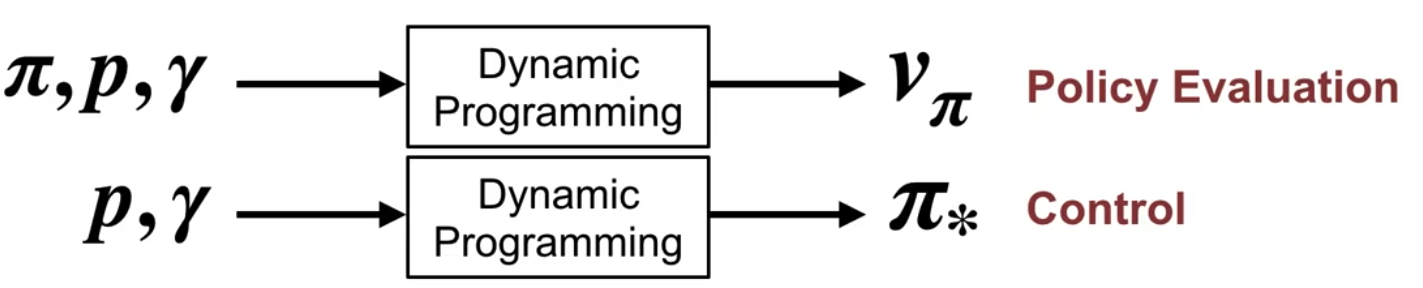
\includegraphics[scale = 0.3]{policy_evaluation_control.png}}
\end{minipage}
\caption{\footnotesize{\textbf{Policy evaluation (Prediction) vs. Control (Policy improvement)}}}
\label{fig: policy_evaluation_control}
\end{figure}


\underline{Control is the ultimate goal of reinforcement learning}. But the task of policy evaluation is usually a necessary first step. It's hard to improve our policy if we don't have a way to assess how good it is. This chapter, we will look at a collection of algorithms called \emph{\textbf{dynamic programming (DP)}} for solving both policy evaluation and control problems.

\emph{Dynamic programming algorithms} use the \emph{Bellman equations} to define iterative algorithms for both policy evaluation and control.  Recall the \emph{Bellman equation} for value function $v$ and action-value function $q$: 
\begin{align}
v_{\pi}(s) &=  \sum_{a}\pi(a|s)\sum_{s'}\sum_{r}p(s', r| s, a)\brac{r + \gamma v_{\pi}(s')}, \quad \forall\,\; s\in \cS \label{eqn: bellman_eqn_value} \\
&= \E{}{R_{t+1}  + \gamma\,v_{\pi}(S_{t+1}) | S_{t} = s} \label{eqn: bellman_eqn_value3}\\
q_{\pi}(s, a) &=\sum_{s', r}p(s', r|s,a)\brac{r+ \gamma \sum_{a'}\pi(a'|s')q_{\pi}(s', a')} \label{eqn: bellman_eqn_value_action}\\
&=\E{}{R_{t+1} + \gamma q_{\pi}(S_{t+1}, A_{t+1}) | S_{t}=s, A_{t}=a}  \label{eqn: bellman_eqn_value_action_3}
\end{align}
where $v_{\pi}: \cS \rightarrow \bR$ is value function and $q_{\pi}: \cS \times \cA \rightarrow \bR$ is the action-value function. $r(s, a) := \E{\pi}{R_{t+1}|S_{t}=s, A_{t}=a}$ and $p(s', r| s, a)$ is the dynamic function of the MDP. $p(s'| s, a)$ is the state transition probability. The optimal value $v_{*}$ and $q_{*}$ also follows the \emph{Bellman optimality equation}:
\begin{align}
v_{*}(s) &=  \max_{a\in \cA(s)}\E{}{R_{t+1} + \gamma v_{*}(S_{t+1}) | S_{t}=s, A_{t}=a} \label{eqn: bellman_eqn_optimal_value}\\
&= \max_{a\in \cA(s)}\sum_{s'}\sum_{r}p(s', r|s, a)\brac{r + \gamma v_{*}(s')} \quad s\in \cS \label{eqn: bellman_eqn_optimal_value2} \\
q_{*}(s, a) &=  \E{}{R_{t+1} + \gamma \max_{a'\in \cA(s)}q_{*}(S_{t+1}, a') \Big| S_{t}=s, A_{t}=a} \label{eqn: bellman_eqn_optimal_value_action3}\\
&=\sum_{s'}\sum_{r}p(s', r|s, a)\brac{r + \gamma  \max_{a'\in \cA(s)}q_{*}(s', a')} \quad \forall\,\; s\in \cS, \; a\in \cA(s) \label{eqn: bellman_eqn_optimal_value_action2}
\end{align} From the Bellman equation, we can see that value function of current state is linearly dependent on the expected rewards and the expected\emph{ values of all successor states}. In other words, the Bellman equation decomposes the original problem into a series of \emph{\textbf{subproblems}} with the \emph{\textbf{same structure}}. This \textbf{recursive structure} is the basis of efficient algorithms such as dynamic programming. In particular, the value function or the optimal value function provides an efficient data structure that allows us to cache the expected long-term future rewards locally at each iteration. The \textbf{key} idea of DP, and of reinforcement learning generally, is the use of \underline{value functions} to organize and structure the \textbf{search} for good policies.


Classical DP algorithms are \underline{of limited utility} in reinforcement learning both because of their assumption of \textbf{a  \underline{perfect model}} (i.e. know dynamic function $p$ for all $s, a, s', r$) and because of their great \emph{\textbf{computational expense}}, but they are still important theoretically. In fact, all of reinforcement learning methods can be viewed as attempts to achieve much the same effect as DP, only with less computation and without assuming a perfect model of the environment.

Compared to brute-force search on $|\cA|^{|\cS|}$ over all possible state-action pairs, dynamic algorithm is \emph{polynomial} in terms of $|\cA|$ and $|\cS|$, which is quite efficient. Thus, dynamic programming is \emph{exponentially faster} than the brute-force search of the policy space.

Generally, solving an MDP gets harder as the number of states grows. The \textbf{curse of dimensionality} says that the size of the state space grows exponentially as the number of state variable increases.  Clearly, this would lead to problems if we try to sweep the states to perform policy iteration.

\section{Policy evaluation (Prediction)}
For given arbitrary policy $\pi$ and dynamic function $p$, the task to compute the value function $v_{\pi}$ is called \textbf{policy evaluation}. From \eqref{eqn: bellman_eqn_value}, we can define an \emph{iterative algorithm} that update the new value function of a state based on the old value function from the successor states, and the expected immediate rewards, along all the one-step transitions possible under the policy being evaluated. 
\begin{align}
v_{t+1}(s) &=    \sum_{a}\pi(a|s)\sum_{s'}\sum_{r}p(s', r| s, a)\brac{r + \gamma v_{t}(s')}, \quad \forall\,\; s\in \cS  \label{eqn: policy_eval_1}
\end{align} Note that the update is an affine mapping, $\mb{v}_{t+1} = \mb{T}\mb{v}_{t} + \mb{r}$, where $\mb{T}$ is determined by $\pi$ and $p$ and $\mb{r}$ is the expected immediate rewards. We call this kind of operation an \emph{expected update}, because they are based on an expectation over \emph{all possible next states} rather than on a sample next state.

if $\mb{r}=\mb{0}$, MDP becomes random walk. The iterative algorithm \eqref{eqn: policy_eval_1} is essentially \textbf{Page-Rank algorithm}  \eqref{eqn: policy_eval_1} converges to a fix-point solution $\mb{v}_{t} = \mb{v}_{\pi}$ which follows the Bellman equation. The bias term $\mb{r}$ is the expected rewards, which accumulates during the iteration, making sure the value function approximates  the goal of reinforcement learning. 

The algorithm for in-place policy evaluation algorithm is described in Figure \ref{fig: policy_evaluation_dp}. Formally, iterative policy evaluation converges only in the limit, but in practice it must be halted short of this. The pseudocode tests the quantity $\max_{s\in \cS} |v_{k+1}(s)-v_{k}(s)|$ after each sweep and stops when it is sufficiently small. We think of the updates as being done \emph{in a \textbf{sweep}} through the state space. For the in-place algorithm, the order in which states have their values updated during the sweep has a significant influence on the rate of convergence. We usually have the in-place version in mind when we think of DP algorithms.
\begin{figure}
\begin{minipage}[t]{1\linewidth}
  \centering
  \centerline{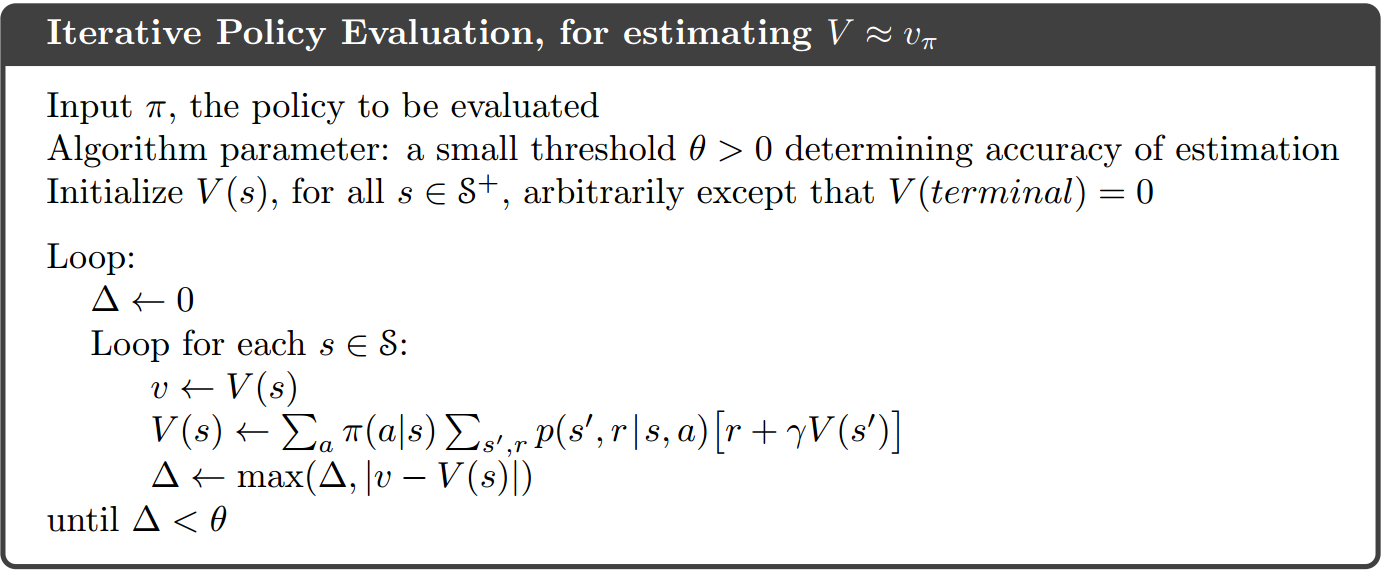
\includegraphics[scale = 0.3]{policy_evaluation_dp.png}}
\end{minipage}
\caption{\footnotesize{\textbf{Policy evaluation  \citep{sutton2018reinforcement}}}}
\label{fig: policy_evaluation_dp}
\end{figure}

\section{Policy Iteration (Control)}
\begin{figure}
\begin{minipage}[t]{1\linewidth}
  \centering
  \centerline{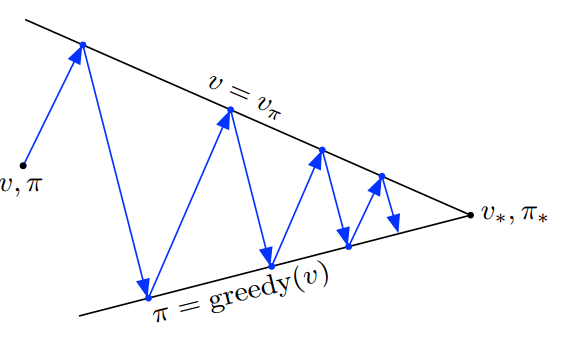
\includegraphics[scale = 0.3]{policy_iteration.png}}
\end{minipage}
\caption{\footnotesize{\textbf{Policy iteration}}}
\label{fig: policy_iteration}
\end{figure}


Our reason for computing the value function for a policy is to help find better policies. For an arbitrary policy $\pi$, how to an improved policy $\pi'$ so that $\pi' \ge \pi$ for every state ?  One way to answer this question is to consider selecting $a$ in $s$ and thereafter following the existing policy, $\pi$. The value of this way of behaving is
\begin{align*}
q_{\pi}(s, a) &= \E{}{R_{t+1} + \gamma\,v_{\pi}(S_{t+1}) | S_{t}=s, A_{t}=a} \\
&= \sum_{s', r}p(s', r | s, a)\brac{r+ \gamma v_{\pi}(s')}
\end{align*} In fact, given policy $\pi$ and action-value $q$, we have the following \emph{\textbf{policy improvement theorem}}
\begin{theorem} (\textbf{Policy improvement theorem})
Let $\pi$ and $\pi'$ be any pair of deterministic policies such that, for all $s \in \cS$, 
\begin{align}
q_{\pi}(s, \pi'(s)) &\ge v_{\pi}(s). \label{eqn: policy_improv_theorem_1}
\end{align}
Then the policy $\pi'$ must be\textbf{ as good as, or better than}, $\pi$. That is, it must obtain greater or equal expected return from all states $s \in \cS$:
\begin{align}
v_{\pi'}(s) &\ge v_{\pi}(s).  \label{eqn: policy_improv_theorem_2}
\end{align} Moreover, if there is strict inequality of \eqref{eqn: policy_improv_theorem_1} at any state, then there must be strict inequality of \eqref{eqn: policy_improv_theorem_2} at that state. 
\end{theorem}
\begin{proof}
The idea behind the proof of the policy improvement theorem is easy to understand. Starting from \eqref{eqn: policy_improv_theorem_1}, we keep expanding the $q_{\pi}$ side with \eqref{eqn: bellman_eqn_value_action}  and reapplying \eqref{eqn: policy_improv_theorem_1} until we get $v_{\pi'}(s)$:
\begin{align*}
v_{\pi}(s) &\le  q_{\pi}(s, \pi'(s)) \\
&=  \E{}{R_{t+1} + \gamma\,v_{\pi}(S_{t+1}) | S_{t}=s, A_{t}=\pi'(s)} \\
&=  \E{\pi'}{R_{t+1} + \gamma\,v_{\pi}(S_{t+1}) | S_{t}=s} \\
&\le  \E{\pi'}{R_{t+1} + \gamma\,q_{\pi}(S_{t+1}, \pi'(S_{t+1})) | S_{t}=s} \\
&=  \E{\pi'}{R_{t+1} + \gamma\, \E{}{R_{t+2} + \gamma\,v_{\pi}(S_{t+2}) | S_{t+1}, A_{t+1}=\pi'(S_{t+1})} | S_{t}=s} \\
&=  \E{\pi'}{\E{}{R_{t+1} + \gamma\,R_{t+2} + \gamma^{2}\,v_{\pi}(S_{t+2}) | S_{t+1}, A_{t+1}=\pi'(S_{t+1})} | S_{t}=s} \\
&=  \E{\pi'}{R_{t+1} + \gamma\,R_{t+2} + \gamma^{2}\,v_{\pi}(S_{t+2}) | S_{t}=s} \\
&\le \E{\pi'}{R_{t+1} + \gamma\,R_{t+2} + \gamma^{2}\,R_{t+3} + \gamma^{3} v_{\pi}(S_{t+3}) | S_{t}=s} \\
&\ldots \\
&\le \E{\pi'}{R_{t+1} + \gamma\,R_{t+2} + \gamma^{2}\,R_{t+3} + \ldots | S_{t}=s} \\
&= \E{\pi'}{G_{t} | S_{t}=s} \\
&= v_{\pi'}(s).
\end{align*} \QEDB
\end{proof}
So far we have seen how, given a policy and its value function, we can easily evaluate a change in the policy at a single state to a particular action. It is a natural extension to consider changes at all states and to all possible actions, selecting at each state the action that appears best according to $q_{\pi}(s, a)$. So frr, we only consider the deterministic policy $\pi(s)$, but the proof holds for stochastic policy $\pi(a|s)$.

\begin{figure}
\begin{minipage}[t]{1\linewidth}
  \centering
  \centerline{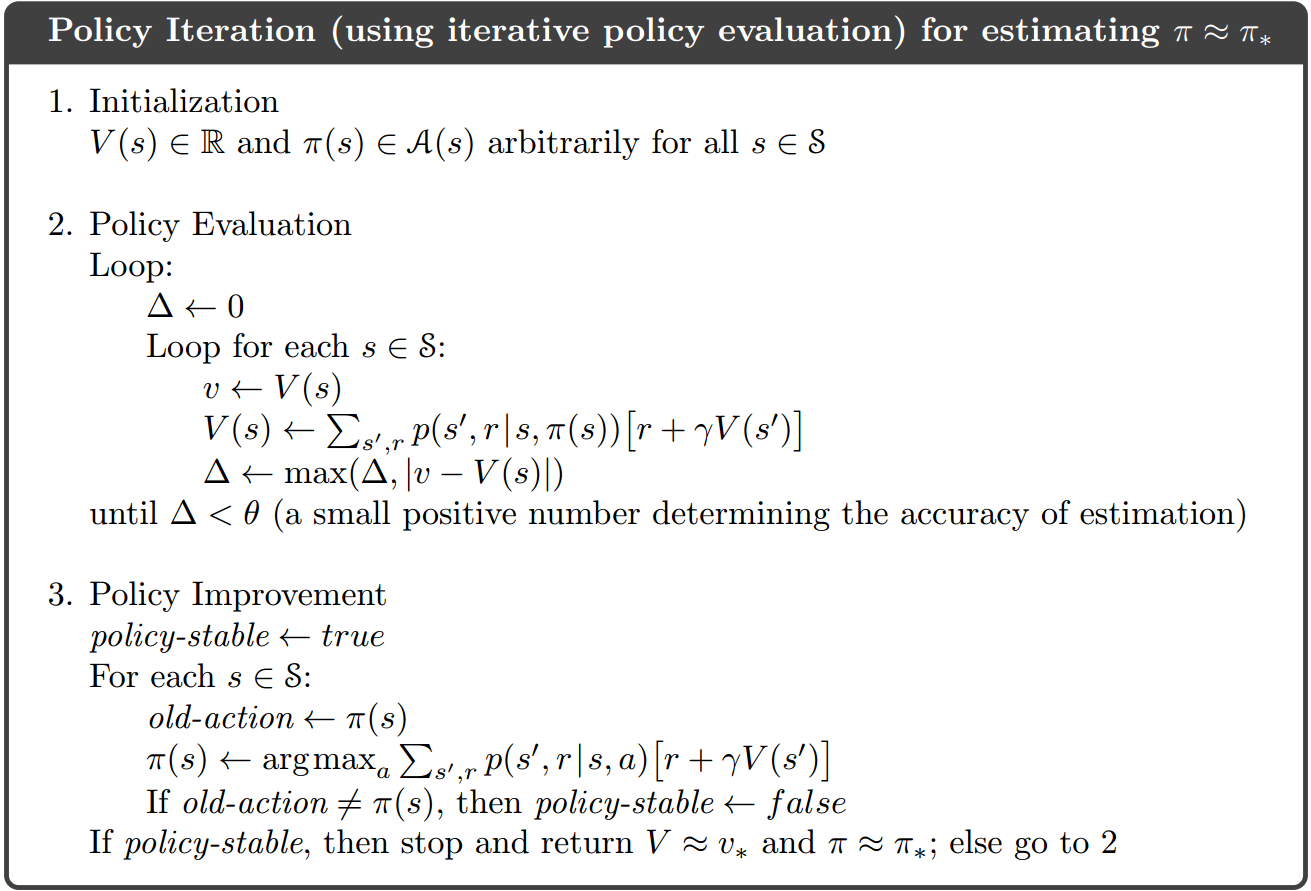
\includegraphics[scale = 0.3]{policy_iter_algo.png}}
\end{minipage}
\caption{\footnotesize{\textbf{Policy iteration Algorithm}}}
\label{fig: policy_iteration_algo}
\end{figure}

Given $\pi_{t}$ and action-value function $q$ or value function $v$, a new policy $\pi_{t+1}$ can be obtained via \textbf{greedy algorithm} 
\begin{align}
\pi_{t+1}(s) &= \argmax_{a \in \cA(s)}q_{\pi_{t}}(s, a), \quad \forall\,\; s\in \cS \nonumber\\
&= \argmax_{a \in \cA(s)}\sum_{s'}\sum_{r}p(s', r| s, a)\brac{r + \gamma\,v_{\pi_{t}}(s')} \;\; (\text{via \eqref{eqn: bellman_eqn_value_action}}) \label{eqn: policy_iter_1}
\end{align} \eqref{eqn: policy_iter_1} is a greedy algorithm at given state $s$, the action selected by the new policy $\pi_{t+1}$ is to maximize the local value function. The greedy  policy $\pi_{t+1}$ takes the action that looks \textbf{best} in the short term -- \emph{after one step of lookahead} -- according to $v$.  ($\pi_{t+1}$ is deterministic if the max is uniquely obtained; otherwise, it can select each optimal action with equal probability.) 

Suppose the new greedy policy, $\pi'$, is as good as, but not better than, the old policy $\pi$. Then $v_{\pi'}(s) = v_{\pi}(s)$. When the algorithm coverges, the Bellman optimality equation is satisfied.  Figure \ref{fig: policy_iteration_algo} describes the policy iteration algorithm by combining both the policy evaluation in Figure \ref{fig: policy_evaluation_dp} and the policy improvement in \eqref{eqn: policy_iter_1}. 


Once a policy, $\pi$, has been improved using $v$ to yield a better policy, $\pi'$, we can then compute $v'$ and improve it again to yield an even better $\pi''$. We can thus obtain a sequence of monotonically improving policies and value functions:
\begin{align*}
\pi_{0} \xrightarrow{E} v_{\pi_0} \xrightarrow{I} \pi_{1} \xrightarrow{E} v_{\pi_1}  \xrightarrow{I} \ldots \xrightarrow{I} \pi_{*} \xrightarrow{E} v_{*}
\end{align*} where $ \xrightarrow{E}$ denotes a policy evaluation and $\xrightarrow{I}$ denotes a policy improvement. Each policy is guaranteed to be a strict improvement over the previous one (unless it is already optimal). Because a finite MDP has only a finite number of policies, this process must converge to an optimal policy and optimal value function in a finite number of iterations. This way of finding an optimal policy is called \underline{\emph{\textbf{policy iteration}}}.




\section{Value iteration} 
One drawback to policy iteration is that each of its iterations involves \emph{policy evaluation}, which may itself be a protracted iterative computation requiring \textbf{multiple sweeps through the state set}. In fact, policy evaluation can be stopped after just one sweep (one update of each state). This algorithm is called \textit{\textbf{value iteration}}. 

\begin{align}
v_{t+1}(s)&=  \max_{a\in \cA(s)}\brac{r(s, a) + \gamma \sum_{s'}p(s'|s, a)v_{t}(s')} \label{eqn: value_iter_1}\\
&= \max_{a\in \cA(s)}\sum_{s'}\sum_{r}p(s', r|s, a)\brac{r + \gamma v_{t}(s')} \quad s\in \cS \label{eqn: value_iter_2}
\end{align} Compare \eqref{eqn: value_iter_2} and \eqref{eqn: policy_iter_1}, we can see that instead of computing $v_{\pi}$ from old policy $\pi$ to update $\pi'$, which from \eqref{eqn: policy_eval_1} requires averaging over all possible actions, we can directly use the old value $v_{t}$ to update new value $v_{t+1}$. Similar to the convergence proof for policy iteration, for arbitrary $v_{0}$, the sequence $\{v_k\}$ can be shown to converge to $v_{*}$ under the same conditions that guarantee the existence of $v_{*}$, i.e. the Bellman optimality equation. Given $v_{*}$, $\pi_{*}$ can be obtained via greedy algorithm in \eqref{eqn: policy_iter_1}.

Another way of understanding value iteration is by reference to the Bellman optimality equation \eqref{eqn: bellman_eqn_optimal_value} and \eqref{eqn: bellman_eqn_optimal_value2}. Note that value iteration is obtained simply by turning the Bellman optimality equation into an update rule. 

Finally, let us consider how value iteration terminates. Like policy evaluation, value iteration formally requires an infinite number of iterations to converge exactly to $v_{*}$. In
practice, we stop once the value function changes by only a small amount in a sweep. The Figure \ref{fig: value_iter_algo} shows a complete algorithm with this kind of termination condition.
\begin{figure}
\begin{minipage}[t]{1\linewidth}
  \centering
  \centerline{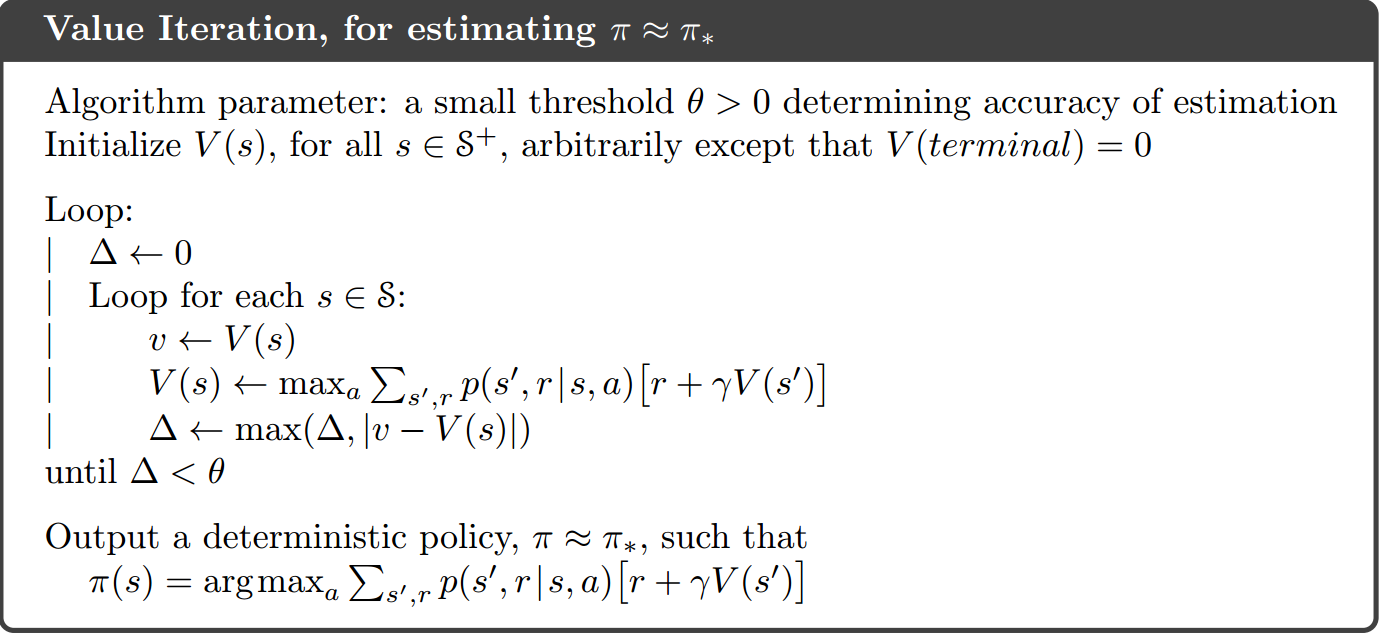
\includegraphics[scale = 0.3]{value_iter_algo.png}}
\end{minipage}
\caption{\footnotesize{\textbf{Value iteration Algorithm}}}
\label{fig: value_iter_algo}
\end{figure}


\section{Generalized Policy Iteration}
Policy iteration consists of two simultaneous, interacting processes, one making the value function consistent with the current policy (policy evaluation), and the other making
the policy greedy with respect to the current value function (policy improvement). In policy iteration, these two processes alternate, each completing before the other begins,
but this is not really necessary. In value iteration, for example, only a single iteration of policy evaluation is performed in between each policy improvement. In asynchronous DP
methods, the evaluation and improvement processes are interleaved at an even finer grain.

We use the term \textbf{generalized policy iteration (GPI)} to refer to the general idea of letting policy-evaluation and policyimprovement processes interact, independent of the granularity and other details of the two processes. Almost all reinforcement learning methods are well described as GPI. That is, all have identifiable policies and value functions, with the policy always being improved with respect to the value function and the value function always being driven toward the value function for the policy, as suggested by the diagram to the right. If both the evaluation process and the improvement process stabilize, that is, no longer produce changes, then the value function and policy
must be optimal.  Figure \ref{fig: GPI} shows this idea. 
\begin{figure}
\begin{minipage}[t]{1\linewidth}
  \centering
  \centerline{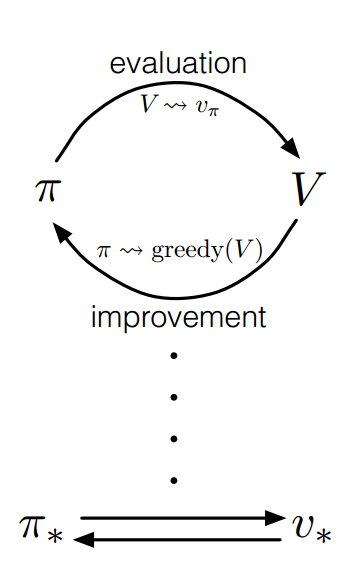
\includegraphics[scale = 0.3]{GPI.png}}
\end{minipage}
\caption{\footnotesize{\textbf{Generalized Policy iteration}}}
\label{fig: GPI}
\end{figure}

The evaluation and improvement processes in GPI can be viewed as both \emph{competing} and \emph{cooperating}. They compete in the sense that they pull in opposing directions. Making the policy greedy with respect to the value function typically makes the value function incorrect for the changed policy, and making the value function consistent with the policy typically causes that policy no longer to be greedy. In the long run, however, these two processes interact to find a single joint solution: the optimal value function and an optimal policy.

Note that this \emph{Generalized Policy Iteration} is an iterative algorithm with two steps: \textbf{policy evaluation} and \textbf{control}, which is similar to \emph{Expectation-Maximization (\textbf{EM}) algorithm} in statistics/supervised learning. EM algorithm is an iterative algorithm with two steps: \emph{expectation} or \textbf{inference} and \emph{maximization} or \textbf{learning}. In fact, the control step in GPI is equivalent to the learning step in EM, since both involves finding optimal model (policy vs. model parameter) that maximizing the objective function (expected value vs. log-likelihood function).  Similarly, the policy evaluation step in GPI is equivalent to the expectation/inference step in EM, since both involves estimating the statistics via taking expectation (value function vs. complete log-likelihood function). Similar to EM algorithm, policy iteration provides a way of heuristic search for optimal policy and optimal value simultaneously. 


\newpage
\bibliographystyle{plainnat}
\bibliography{reference.bib}
\end{document}